\documentclass[xetex,mathserif,serif]{beamer}
\usepackage{polyglossia}
\setdefaultlanguage[babelshorthands=true]{russian}
\usepackage{minted}
\usepackage{tabu}

\useoutertheme{infolines}

\usepackage{fontspec}
\setmainfont{FreeSans}
\newfontfamily{\russianfonttt}{FreeSans}

\tabulinesep=0.7mm

\title{Порождающие и поведенческие паттерны, детали реализации}
\author[Юрий Литвинов]{Юрий Литвинов \newline \textcolor{gray}{\small\texttt{yurii.litvinov@gmail.com}}}

\date{10.04.2019г}

\begin{document}
	
	\frame{\titlepage}

	\section{Порождающие шаблоны}

	\begin{frame}
		\frametitle{``Фабричный метод'' (Factory Method), детали реализации}
		\begin{center}
			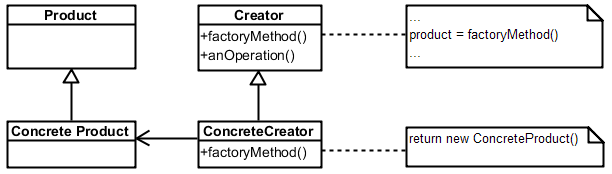
\includegraphics[width=0.6\textwidth]{factoryMethod.png}
		\end{center}
		\begin{itemize}
			\item Абстрактный Creator или реализация по умолчанию
			\begin{itemize}
				\item Второй вариант может быть полезен для расширяемости
			\end{itemize}
			\item Параметризованные фабричные методы
			\item Если язык поддерживает инстанциацию по прототипу (JavaScript, Smalltalk), можно хранить порождаемый объект
			\item Creator не может вызывать фабричный метод в конструкторе
			\item Можно сделать шаблонный Creator
		\end{itemize}
	\end{frame}

	\begin{frame}
		\frametitle{``Абстрактная фабрика'' (Abstract Factory), детали реализации}
		\begin{columns}
			\begin{column}{0.5\textwidth}
				\begin{itemize}
					\item Хорошо комбинируются с паттерном ``Одиночка''
					\item Если семейств продуктов много, то фабрика может инициализироваться \textit{прототипами}, тогда не надо создавать сотню подклассов
				\end{itemize}
			\end{column}
			\begin{column}{0.5\textwidth}
				\begin{center}
					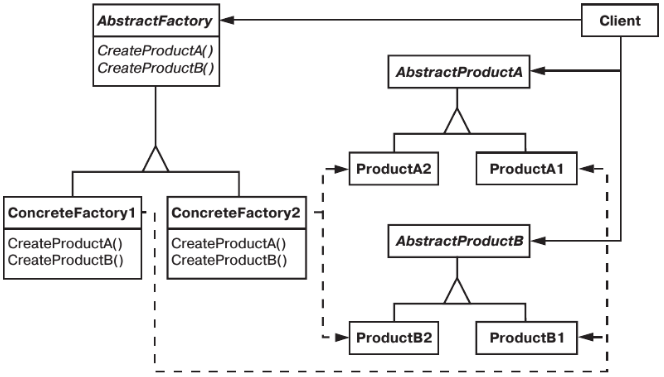
\includegraphics[width=\textwidth]{abstractFactory.png}
				\end{center}
			\end{column}
		\end{columns}
		\begin{itemize}
			\item Прототип на самом деле может быть классом (например, Class в Java)
			\item Если виды объектов часто меняются, может помочь параметризация метода создания
			\begin{itemize}
				\item Может пострадать типобезопасность
			\end{itemize}
		\end{itemize}
	\end{frame}

	\begin{frame}
		\frametitle{``Прототип'' (Prototype), детали реализации}
		\begin{columns}
			\begin{column}{0.45\textwidth}
				\begin{itemize}
					\item Реестр прототипов, обычно ассоциативное хранилище
				\end{itemize}
			\end{column}
			\begin{column}{0.55\textwidth}
				\begin{center}
					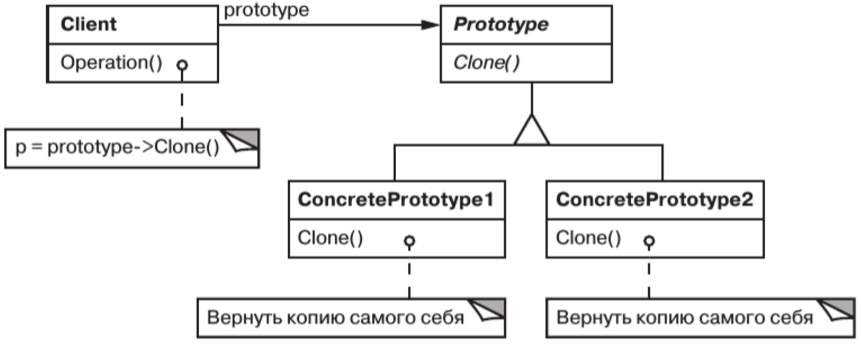
\includegraphics[width=\textwidth]{prototype.png}
				\end{center}
			\end{column}
		\end{columns}
		\begin{itemize}
			\item Операция Clone
			\begin{itemize}
				\item Глубокое и мелкое копирование
				\item В случае, если могут быть круговые ссылки
				\item Сериализовать/десериализовать объект (но помнить про идентичность)
			\end{itemize}
			\item Инициализация клона
			\begin{itemize}
				\item Передавать параметры в Clone --- плохая идея
			\end{itemize}
		\end{itemize}
	\end{frame}

	\begin{frame}
		\frametitle{``Строитель'' (Builder), детали реализации}
		\begin{center}
			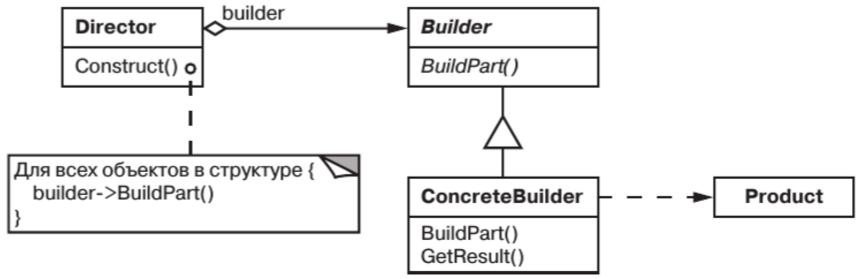
\includegraphics[width=0.7\textwidth]{builder.png}
		\end{center}
		\begin{itemize}
			\item Абстрактные и конкретные строители
			\begin{itemize}
				\item Достаточно общий интерфейс
			\end{itemize}
			\item Общий интерфейс для продуктов не требуется
			\begin{itemize}
				\item Клиент конфигурирует распорядителя конкретным строителем, он же и забирает результат
			\end{itemize}
			\item Пустые методы по умолчанию
		\end{itemize}
	\end{frame}

	\begin{frame}[fragile]
		\frametitle{``Строитель'', примеры}
		\begin{itemize}
			\item StringBuilder
			\item Guava, подсистема работы с графами
			\begin{minted}{java}
MutableNetwork<Webpage, Link> webSnapshot = 
        NetworkBuilder.directed()
    .allowsParallelEdges(true)
    .nodeOrder(ElementOrder.natural())
    .expectedNodeCount(100000)
    .expectedEdgeCount(1000000)
    .build();
			\end{minted}
		\end{itemize}
\end{frame}

	\section{Поведенческие шаблоны}

	\begin{frame}
		\frametitle{``Шаблонный метод'' (Template Method), детали реализации}
		\begin{columns}
			\begin{column}{0.5\textwidth}
				\begin{itemize}
					\item Сам шаблонный метод, как правило, невиртуальный
					\item Лучше использовать соглашения об именовании, например, называть операции с Do
				\end{itemize}
			\end{column}
			\begin{column}{0.4\textwidth}
				\begin{center}
					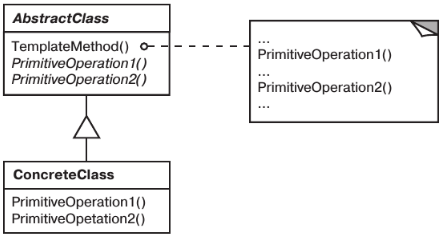
\includegraphics[width=\textwidth]{templateMethod.png}
				\end{center}
			\end{column}
		\end{columns}
		\begin{itemize}
			\item Примитивные операции могут быть виртуальными или чисто виртуальными
			\begin{itemize}
				\item Лучше их делать protected
				\item Чем их меньше, тем лучше
			\end{itemize}
		\end{itemize}
	\end{frame}

	\begin{frame}
		\frametitle{``Посредник'' (Mediator), детали реализации}
		\begin{columns}
			\begin{column}{0.5\textwidth}
				\begin{itemize}
					\item Абстрактный класс ``Mediator'' часто не нужен
					\item Паттерн ``Наблюдатель'': медиатор подписывается на события в коллегах
					\item Наоборот: коллеги вызывают методы медиатора
				\end{itemize}
			\end{column}
			\begin{column}{0.5\textwidth}
				\begin{center}
					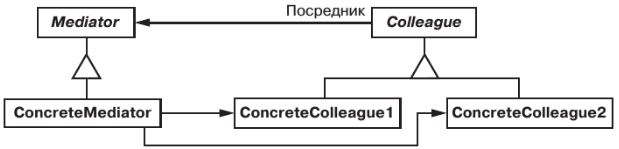
\includegraphics[width=\textwidth]{mediatorClasses.png}
					\vspace{1cm}
					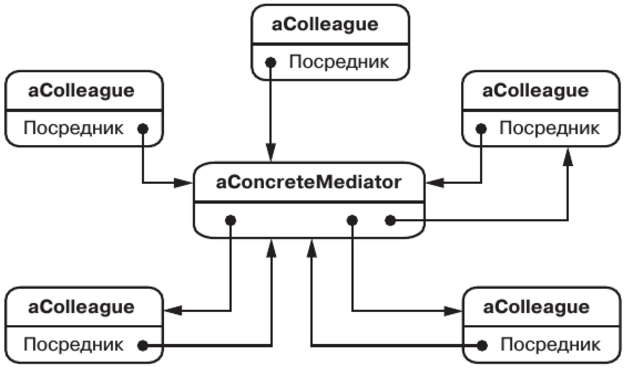
\includegraphics[width=\textwidth]{mediatorObjects.png}
				\end{center}
			\end{column}
		\end{columns}
	\end{frame}

	\begin{frame}
		\frametitle{``Команда'' (Command), детали реализации}
		\begin{center}
			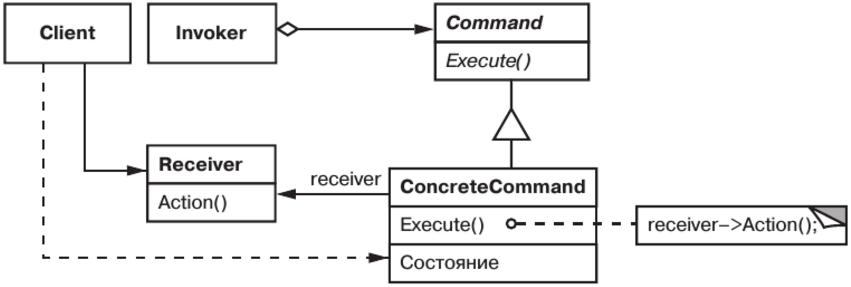
\includegraphics[width=0.6\textwidth]{command.png}
		\end{center}
		\begin{itemize}
			\item Насколько ``умной'' должна быть команда
			\item Отмена и повторение операций --- тоже от хранения всего состояния в команде до ``вычислимого'' отката
			\begin{itemize}
				\item Undo-стек и Redo-стек
				\item Может потребоваться копировать команды
				\item ``Искусственные'' команды
				\item Композитные команды
			\end{itemize}
			\item Паттерн ``Хранитель'' для избежания ошибок восстановления
		\end{itemize}
	\end{frame}

	\begin{frame}[fragile]
		\frametitle{``Команда'', пример}
		\begin{itemize}
			\item Qt, класс QAction:
			\begin{minted}{c++}
const QIcon openIcon = QIcon(":/images/open.png");
QAction *openAct = new QAction(openIcon, tr("&Open..."), this);

openAct->setShortcuts(QKeySequence::Open);
openAct->setStatusTip(tr("Open an existing file"));

connect(openAct, &QAction::triggered, this, &MainWindow::open);

fileMenu->addAction(openAct);
fileToolBar->addAction(openAct);
			\end{minted}
		\end{itemize}
\end{frame}

	\begin{frame}
		\frametitle{``Цепочка ответственности'' (Chain of Responsibility), детали реализации}
		\begin{columns}
			\begin{column}{0.5\textwidth}
				\begin{itemize}
					\item Необязательно реализовывать связи в цепочке специально
					\begin{itemize}
						\item На самом деле, чаще используются существующие связи
					\end{itemize}

				\end{itemize}
			\end{column}
			\begin{column}{0.5\textwidth}
				\begin{center}
					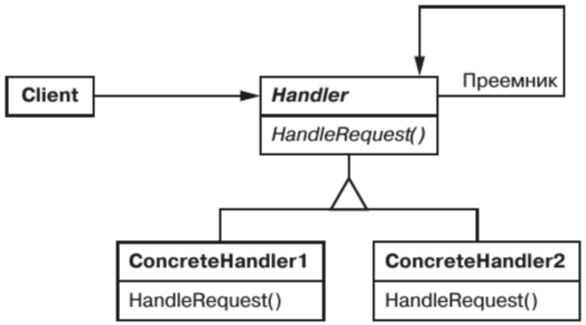
\includegraphics[width=\textwidth]{chainOfResponsibility.png}
				\end{center}
			\end{column}
		\end{columns}
		\begin{itemize}
			\item По умолчанию в Handler передавать запрос дальше (если ссылки на преемника всё-таки есть)
			\item Если возможных запросов несколько, их надо как-то различать
			\begin{itemize}
				\item Явно вызывать методы --- нерасширяемо
				\item Использовать объекты-запросы
			\end{itemize}
		\end{itemize}
	\end{frame}

	\begin{frame}[fragile]
		\frametitle{``Цепочка ответственности'', примеры}
		\begin{itemize}
			\item Распространение исключений
			\item Распространение событий в оконных библиотеках:
			\begin{minted}{c++}
void MyCheckBox::mousePressEvent(QMouseEvent *event)
{
    if (event->button() == Qt::LeftButton) {
        // handle left mouse button here
    } else {
        // pass on other buttons to base class
        QCheckBox::mousePressEvent(event);
    }
}
			\end{minted}
		\end{itemize}
	\end{frame}

	\begin{frame}
		\frametitle{``Наблюдатель'' (Observer), детали реализации}
		\begin{itemize}
			\item В ``нормальных'' языках поддержан ``из коробки'' (через механизм событий)
		\end{itemize}
		\begin{columns}
			\begin{column}{0.45\textwidth}
				\begin{itemize}
					\item Могут использоваться хеш-таблицы для отображения субъектов и наблюдателей
					\begin{itemize}
						\item Так делает WPF в .NET, есть даже языковая поддержка в C\#
					\end{itemize}
				\end{itemize}
			\end{column}
			\begin{column}{0.55\textwidth}
				\begin{center}
					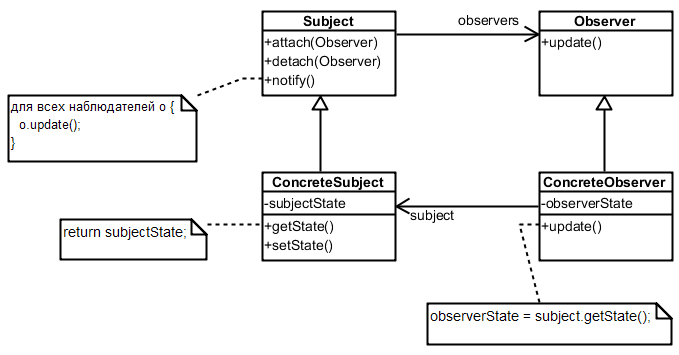
\includegraphics[width=\textwidth]{observer.png}
				\end{center}
			\end{column}
		\end{columns}
		\begin{itemize}
			\item Необходимость идентифицировать субъект
			\item Кто инициирует нотификацию
			\begin{itemize}
				\item Операции, модифицирующие субъект
				\item Клиент, после серии модификаций субъекта
			\end{itemize}
		\end{itemize}
	\end{frame}

		\begin{frame}
		\frametitle{``Наблюдатель'' (Observer), детали реализации (2)}
		\begin{itemize}
			\item Ссылки на субъектов и наблюдателей
			\begin{itemize}
				\item Простой способ организовать утечку памяти в C\# или грохнуть программу в C++
			\end{itemize}
			\item Консистентность субъекта при отправке нотификации
			\begin{itemize}
				\item Очевидно, но легко нарушить, вызвав метод предка в потомке
				\item ``Шаблонный метод''
				\item Документировать, кто когда какие события бросает
			\end{itemize}
			\item Передача сути изменений --- pull vs push
			\item Фильтрация по типам событий
			\item Менеджер изменений (``Посредник'')
		\end{itemize}
	\end{frame}

	\begin{frame}[fragile]
		\frametitle{``Наблюдатель'', пример (1)}
		\begin{itemize}
			\item События в C\#:
			\begin{minted}{csharp}
internal class NewMessageEventArgs : EventArgs {
    private readonly string message;

    public MessageEventArgs(string message) 
        => this.message = message;

    public string Message => message;
}
			\end{minted}
		\end{itemize}
\end{frame}

	\begin{frame}[fragile]
		\frametitle{``Наблюдатель'', пример (2)}
		\begin{small}
			\begin{minted}{csharp}
internal class Messenger {
    public event EventHandler<NewMessageEventArgs> NewMessage;

    protected virtual void OnMessage(NewMessageEventArgs e) {
        EventHandler<NewMessageEventArgs> temp 
                = Volatile.Read(ref NewMessage);
        if (temp != null) 
            temp(this, e);
    }

    public void SimulateMessage(String message) {
        var e = new NewMessageEventArgs(message);
        OnMessage(e);
    }
}
			\end{minted}
		\end{small}
\end{frame}

	\begin{frame}[fragile]
		\frametitle{``Наблюдатель'', пример (3)}
		\begin{itemize}
			\begin{minted}{csharp}
internal sealed class Fax {
    public Fax(Messenger mm) => mm.NewMessage += FaxMsg;

    private void FaxMsg(object sender, NewMessageEventArgs e) {
        Console.WriteLine("Faxing message:");
        Console.WriteLine($"Message={e.Message}");
    }

    public void Unregister(Messenger mm) 
        => mm.NewMessage -= FaxMsg;
}
			\end{minted}
		\end{itemize}
\end{frame}

	\begin{frame}
		\frametitle{``Состояние'' (State), детали реализации}
		\begin{columns}
			\begin{column}{0.5\textwidth}
				\begin{itemize}
					\item Переходы между состояниями --- в Context или в State?
					\item Таблица переходов
					\begin{itemize}
						\item Трудно добавить действия по переходу
					\end{itemize}
				\end{itemize}
			\end{column}
			\begin{column}{0.5\textwidth}
				\begin{center}
					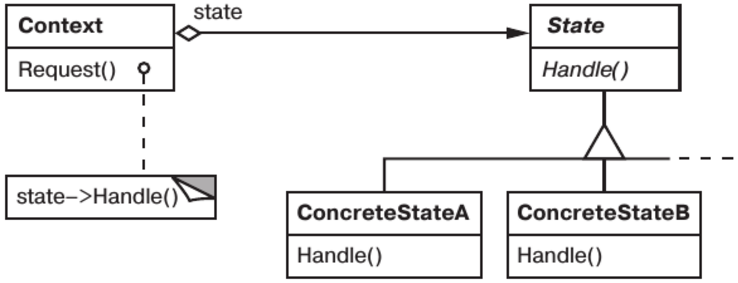
\includegraphics[width=\textwidth]{state.png}
				\end{center}
			\end{column}
		\end{columns}
		\begin{itemize}
			\item Создание и уничтожение состояний
			\begin{itemize}
				\item Создать раз и навсегда
				\item Создавать и удалять при переходах
			\end{itemize}
		\end{itemize}
	\end{frame}

	\begin{frame}
		\frametitle{``Посетитель'' (Visitor), детали реализации}
		\begin{columns}
			\begin{column}{0.4\textwidth}
				\begin{itemize}
					\item Использовать перегрузку методов Visit(...)
					\item Чаще всего сама коллекция отвечает за обход, но может быть итератор
					\item Может даже сам Visitor, если обход зависит от результата операции
				\end{itemize}
			\end{column}
			\begin{column}{0.6\textwidth}
				\begin{center}
					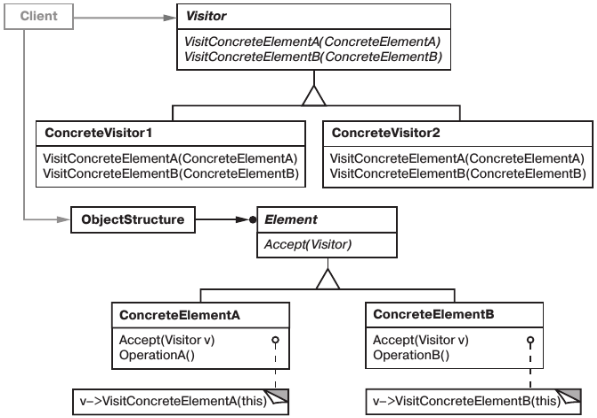
\includegraphics[width=\textwidth]{visitor.png}
				\end{center}
			\end{column}
		\end{columns}
	\end{frame}

% 	\begin{frame}[fragile]
% 		\frametitle{``Посетитель'', пример}
% 		\begin{itemize}
% 			\begin{minted}{csharp}
% 				Здесь будет пример кода на ANTLR
% 			\end{minted}
% 		\end{itemize}
% \end{frame}

	\begin{frame}
		\frametitle{``Хранитель'' (Memento), детали реализации}
		\begin{center}
			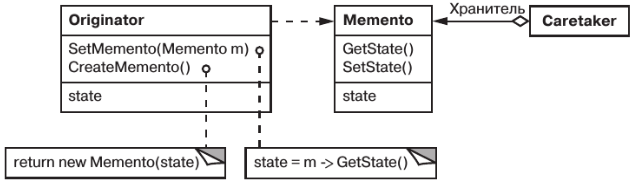
\includegraphics[width=0.7\textwidth]{memento.png}
		\end{center}
		\begin{itemize}
			\item Два интерфейса: ``широкий'' для хозяев и ``узкий'' для остальных объектов
			\begin{itemize}
				\item Требуется языковая поддержка
			\end{itemize}
			\item Можно хранить только дельты состояний
		\end{itemize}
	\end{frame}

	\begin{frame}
		\frametitle{``Интерпретатор'' (Interpreter)}
		Определяет представление грамматики и интерпретатор для заданного языка.
		\begin{center}
			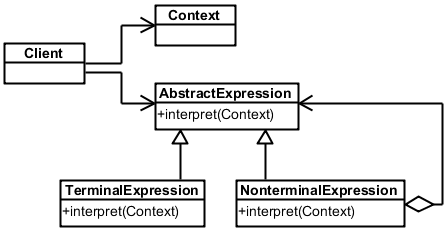
\includegraphics[width=0.6\textwidth]{interpreter.png}
		\end{center}
		\begin{itemize}
			\item Грамматика должна быть проста (иначе лучше ``Visitor'')
			\item Эффективность не критична
		\end{itemize}
	\end{frame}

	\begin{frame}
		\frametitle{``Интерпретатор'', пример}
		\begin{center}
			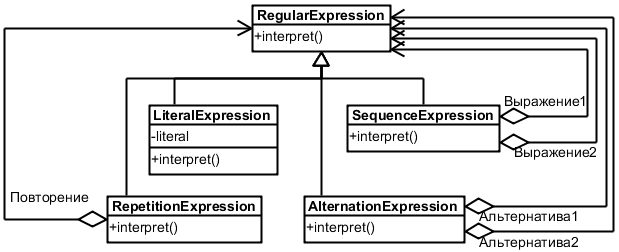
\includegraphics[width=0.8\textwidth]{regexp.png}
		\end{center}
	\end{frame}

	\begin{frame}
		\frametitle{``Интерпретатор'', детали реализации}
		\begin{footnotesize}
			\textbf{10-е правило Гринспена:}
			
			\textit{Любая достаточно сложная программа на Си или Фортране содержит заново написанную, неспецифицированную, глючную и медленную реализацию половины языка Common Lisp}
		\end{footnotesize}
		\begin{itemize}
			\item Построение дерева --- отдельная задача
			\item Несколько разных операций над деревом --- лучше ``Visitor''
			\item Можно использовать ``Приспособленец'' для разделения терминальных символов
		\end{itemize}
	\end{frame}

	\begin{frame}
		\frametitle{``Итератор'' (Iterator)}
		Инкапсулирует способ обхода коллекции.
		\begin{center}
			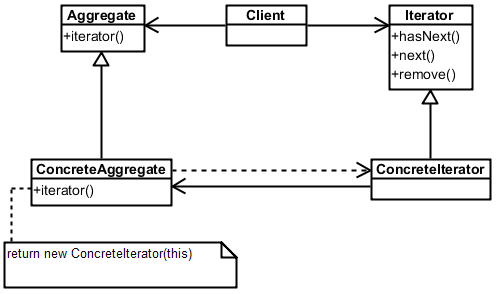
\includegraphics[width=0.6\textwidth]{iterator.png}
		\end{center}
		\begin{itemize}
			\item Разные итераторы для разных способов обхода
			\item Можно обходить не только коллекции
		\end{itemize}
	\end{frame}

	\begin{frame}[fragile]
		\frametitle{``Итератор'', примеры}
		\begin{itemize}
			\item Java-стиль:
			\begin{minted}{java}
public interface Iterator<E> {
    boolean hasNext();
    E next();
    void remove();
}
			\end{minted}
			\item .NET-стиль:
			\begin{minted}{csharp}
public interface IEnumerator<T>
{
    bool MoveNext();
    T Current { get; }
    void Reset();
}
			\end{minted}
		\end{itemize}
	\end{frame}

	\begin{frame}[fragile]
		\frametitle{``Итератор'', детали реализации (1)}
		\begin{itemize}
			\item Внешние итераторы
			\begin{minted}{csharp}
foreach (Thing t in collection)
{
    Console.WriteLine(t);
} 
			\end{minted}
			\item Внутренние итераторы
			\begin{minted}{csharp}
collection.ToList().ForEach(t => Console.WriteLine(t));
			\end{minted}
		\end{itemize}
\end{frame}

	\begin{frame}
		\frametitle{``Итератор'', детали реализации (2)}
		\begin{itemize}
			\item Итераторы и курсоры
			\item Устойчивые и неустойчивые итераторы
			\begin{itemize}
				\item Паттерн ``Наблюдатель''
				\item Даже обнаружение модификации коллекции может быть непросто
			\end{itemize}
			\item Дополнительные операции
			\item В C++ итераторы --- это сложно
		\end{itemize}
	\end{frame}

\end{document}